\documentclass[12pt,a4paper]{article}

% ------------------------------------------------
% Pacotes Fundamentais
% ------------------------------------------------
\usepackage[utf8]{inputenc}
\usepackage[T1]{fontenc}
\usepackage[brazil]{babel}
\usepackage{graphicx}
\usepackage[table]{xcolor}
\usepackage{array}
\usepackage{tabularx}
\usepackage{geometry}
\usepackage{fancyhdr}
\usepackage{mathptmx} % Times New Roman
\usepackage{enumitem} 
\usepackage{amsfonts}
\usepackage{amsmath}
\usepackage{amssymb}
\usepackage{tikz}
\usetikzlibrary{positioning, shapes.geometric, calc}

% Cores Institucionais
\definecolor{maincolor}{RGB}{0,100,50}
\definecolor{forestgreen}{RGB}{0,100,50}

% ------------------------------------------------
% Estilos TikZ para Diagramas ER, Lógicos e Wireframes CRUD
% ------------------------------------------------
\tikzset{
    block/.style={rectangle, draw=forestgreen, thick, minimum width=2.5cm, minimum height=0.9cm, fill=white, align=center, font=\small\bfseries},
    diamond_node/.style={diamond, draw=forestgreen, thick, minimum width=1.8cm, minimum height=0.9cm, fill=white, aspect=2, align=center, font=\small},
    attribute/.style={ellipse, draw=forestgreen, thin, minimum width=1.6cm, minimum height=0.6cm, fill=white, align=center, font=\scriptsize},
    line/.style={draw, thick, -},
    table_block/.style={
        rectangle, 
        draw=forestgreen, 
        thick, 
        rounded corners=4pt, 
        minimum width=4.5cm, 
        fill=green!2, 
        align=left, 
        font=\small\ttfamily, 
        inner sep=8pt
    },
    screen/.style={draw=forestgreen, thick, rectangle, rounded corners=8pt, minimum width=8.5cm, minimum height=7.0cm, fill=white},
    screen_title/.style={fill=forestgreen, text=white, minimum width=8.3cm, minimum height=0.6cm, font=\footnotesize\bfseries\sffamily, align=center},
    btn/.style={draw=forestgreen, fill=green!10, rounded corners=3pt, font=\tiny\sffamily, inner sep=3pt},
    btn_danger/.style={draw=red, fill=red!10, rounded corners=3pt, font=\tiny\sffamily, inner sep=3pt, text=red},
    input_field/.style={draw=gray!50, fill=gray!2, rectangle, minimum width=7.5cm, minimum height=0.55cm, font=\tiny\sffamily, align=left, inner sep=4pt}
}

% ------------------------------------------------ 
% Configuração de Página e Margens
% ------------------------------------------------
\geometry{
    a4paper,
    left=2cm,
    right=2cm,
    top=2cm,
    bottom=2cm,
    headheight=15pt
}

\pagestyle{fancy}
\fancyhf{}
\renewcommand{\headrulewidth}{0pt}
\setlength{\parindent}{0pt}

% ------------------------------------------------
% Macros Customizadas (Caixa de Resposta e Alinhamento)
% ------------------------------------------------
\newcommand{\resposta}[1]{}

\newcolumntype{L}[1]{>{\raggedright\arraybackslash}p{#1}}
\newcolumntype{C}[1]{>{\centering\arraybackslash}p{#1}}

% ------------------------------------------------
% Configurações de Caixas Decorativas (tcolorbox)
% ------------------------------------------------
\usepackage[most]{tcolorbox}
\newtcolorbox{blockbox}[1]{%
  colback=green!5,
  colframe=forestgreen,
  coltitle=white,
  title=#1,
  fonttitle=\bfseries,
  boxrule=1.5pt,
  arc=3mm,
  left=8pt,
  right=8pt,
  top=8pt,
  bottom=8pt
}

% ------------------------------------------------
% Configurações de Código (Listings SQL)
% ------------------------------------------------
\usepackage{listings}
\definecolor{codegray}{rgb}{0.5,0.5,0.5}
\definecolor{codepurple}{rgb}{0.58,0,0.82}
\definecolor{backcolour}{rgb}{0.96,0.96,0.94}

\lstdefinestyle{sqlstyle}{
    backgroundcolor=\color{backcolour},   
    commentstyle=\color{codegray},
    keywordstyle=\color{forestgreen}\bfseries,
    numberstyle=\tiny\color{codegray},
    stringstyle=\color{codepurple},
    basicstyle=\ttfamily\footnotesize,
    breakatwhitespace=false,         
    breaklines=true,                 
    captionpos=b,                    
    keepspaces=true,                 
    numbers=none,                    
    showspaces=false,                
    showstringspaces=false,
    showtabs=false,                  
    tabsize=2,
    language=SQL,
    morekeywords={REFERENCES, ON, CASCADE, SET, NULL, NO, ACTION, RESTRICT, OFFSET, LIMIT, DISTINCT},
    literate={á}{{\'a}}1 {ã}{{\~a}}1 {â}{{\^a}}1 {à}{{\`a}}1 {é}{{\'e}}1 {ê}{{\^e}}1 {í}{{\'i}}1 {ó}{{\'o}}1 {õ}{{\~o}}1 {ô}{{\^o}}1 {ú}{{\'u}}1 {ç}{{\c{c}}}1 {Á}{{\'A}}1 {Ã}{{\~A}}1 {Â}{{\^A}}1 {À}{{\`A}}1 {É}{{\'E}}1 {Ê}{{\^E}}1 {Í}{{\'I}}1 {Ó}{{\'O}}1 {Õ}{{\~O}}1 {Ô}{{\^O}}1 {Ú}{{\'U}}1 {Ç}{{\c{C}}}1
}
\lstset{style=sqlstyle}

% ================================================
\begin{document}
% ================================================

% ------------------------------------------------
% Cabeçalho Institucional Oficial da UniRV
% ------------------------------------------------
\begin{tabularx}{\textwidth}{@{} L{4.5cm} X @{}}
    \raisebox{-0.5cm}{
\includegraphics[width=4.5cm]{Universidade_de_Rio_Verde.jpg}} &
    \hfill
    \begin{tabular}{|>{\centering\arraybackslash}m{11.6cm}|}
        \hline
        \cellcolor{forestgreen}\color{white}\rule{0pt}{1.2cm}\textbf{ATIVIDADE DE TRATAMENTO EXCEPCIONAL} \tabularnewline
        \hline
    \end{tabular} 
\end{tabularx}
\vspace{0.3cm}

\begin{tabularx}{\textwidth}{|X|L{2.5cm}|}
\hline
\textbf{Curso} & \textbf{Campus} \\
\textit{Engenharia de Software} & \textit{Rio Verde} \\
\hline
\multicolumn{2}{|l|}{\textbf{Disciplina}} \\  
\multicolumn{2}{|l|}{ \textit{Banco de Dados I}} \\
\hline
\textbf{Professor} & \textbf{Turma} \\
\textit{Sergio Souza Novak} & \textit{A / B} \\
\hline
\multicolumn{2}{|l|}{\textbf{Código da Atividade}} \\
\multicolumn{2}{|l|}{\textit{ESW417}} \\
\hline
\end{tabularx}

\vspace{0.5cm}

% ------------------------------------------------
% Seção Introdutória e Orientações para o Colab
% ------------------------------------------------
\begin{blockbox}{Configuração Importante: Google Colab e SQLite}
Para resolver esta lista de exercícios utilizando SQL no \textbf{Google Colab}, certifique-se de executar as etapas iniciais de instalação da extensão SQL e, \textbf{fundamentalmente}, habilitar a integridade referencial de chaves estrangeiras executando o seguinte comando no início do seu notebook:
\begin{center}
    \large\texttt{\%sql PRAGMA foreign\_keys = ON;}
\end{center}
Se essa diretiva não for executada, o SQLite aceitará inserções consistentes de chaves órfãs, prejudicando o teste das restrições DDL formuladas.

\vspace{0.2cm}
\textbf{Instruções de Entrega:} O(a) acadêmico(a) deve resolver todos os exercícios práticos e teóricos propostos e entregar um \textbf{único documento PDF} contendo as respostas e scripts SQL detalhados de todos os exercícios.
\end{blockbox}

\vspace{0.4cm}

\subsection*{A Matemática da Paginação de Dados}
Quando construímos aplicações modernas (aplicativos móveis, dashboards web ou e-commerces), ler milhões de linhas de um banco de dados de uma só vez pode causar sobrecarga de tráfego de rede e congelar a interface do usuário. A técnica de \textbf{Paginação} divide o conjunto de resultados em partes (páginas) controladas.

Em SQL, fazemos isso combinando duas cláusulas avançadas:
\begin{itemize}
    \item \textbf{LIMIT}: Especifica a quantidade máxima de registros a serem retornados na consulta. Corresponde ao tamanho da página.
    \item \textbf{OFFSET}: Especifica o número de registros iniciais que devem ser ignorados (ou "pulados") antes de começar a retornar as linhas.
\end{itemize}

Para implementar a paginação programática, os valores são calculados pelas fórmulas:
\begin{center}
    \large
    \textbf{LIMIT} = $\text{Itens por Página}$ \\
    \textbf{OFFSET} = $(\text{Página Desejada} - 1) \times \text{Itens por Página}$
\end{center}

\textit{Nota crucial}: O uso da cláusula \textbf{ORDER BY} é obrigatório ao usar paginação. Sem ela, o SGDB não garante a ordem das linhas, o que pode causar registros repetidos ou perdidos ao alternar entre as páginas.



% ------------------------------------------------
% EXERCÍCIO 1
% ------------------------------------------------
\section*{Exercíci 1:}

\textbf{Contexto:} Em uma cooperativa agroindustrial em Rio Verde, silos inteligentes de armazenamento de grãos (soja e milho) utilizam sensores IoT para monitorar as condições ambientais a cada hora. Leituras fora dos limites ideais podem causar apodrecimento ou combustão espontânea. O aplicativo móvel do operador exibe um histórico de leituras que precisa ser carregado em páginas de 10 leituras para otimizar a conexão de rede 4G rural.

\begin{center}
    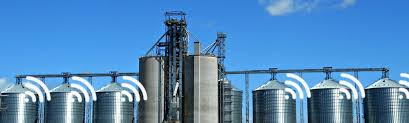
\includegraphics[width=9.5cm, height=5.5cm, keepaspectratio]{silos.jpeg} \\
    \small \textbf{Figura 1.1:} Silos inteligentes de armazenamento de grãos monitorados via sensores IoT.
\end{center}

\vspace{0.3cm}
\begin{center}
    \textbf{Modelo Conceitual (Diagrama Entidade-Relacionamento)} \\[0.2cm]
    \begin{tikzpicture}[node distance=1.5cm, >=stealth, thick, scale=0.9, every node/.style={transform shape}]
        \node[block] (silo) {Silo};
        \node[diamond_node, right=2.2cm of silo] (possui) {Possui};
        \node[block, right=2.2cm of possui] (leitura) {LeituraSilo};
        
        \path[line] (silo) -- (possui);
        \path[line] (possui) -- (leitura);
        
        % Atributos Silo
        \node[attribute, above left=1cm and 0.4cm of silo] (id_silo) {\underline{id\_silo}};
        \node[attribute, left=1.2cm of silo] (ident) {identificador};
        \node[attribute, below left=1cm and 0.4cm of silo] (cap) {capacidade\_ton};
        \node[attribute, above=0.8cm of silo] (loc) {localizacao};
        
        \path[line] (silo) -- (id_silo);
        \path[line] (silo) -- (ident);
        \path[line] (silo) -- (cap);
        \path[line] (silo) -- (loc);
        
        % Atributos LeituraSilo
        \node[attribute, above right=1cm and 0.4cm of leitura] (id_leit) {\underline{id\_leitura}};
        \node[attribute, right=1.2cm of leitura] (dt) {data\_hora};
        \node[attribute, below right=1cm and 0.4cm of leitura] (temp) {temperatura};
        \node[attribute, above=0.8cm of leitura] (umid) {umidade};
        
        \path[line] (leitura) -- (id_leit);
        \path[line] (leitura) -- (dt);
        \path[line] (leitura) -- (temp);
        \path[line] (leitura) -- (umid);
        
        % Cardinalidades
        \node[above, font=\small\bfseries] at ($(silo.east)!0.3!(possui.west)$) {1};
        \node[above, font=\small\bfseries] at ($(leitura.west)!0.3!(possui.east)$) {N};
    \end{tikzpicture}
\end{center}

\begin{center}
    \textbf{Modelo Lógico (Relacional)} \\[0.2cm]
    \begin{tikzpicture}[node distance=1.5cm, >=stealth, thick]
        \node[table_block] (silo_tbl) at (0,0) {
            \textbf{tbSilo} \\
            \rule{4.1cm}{0.4pt} \\
            \underline{id\_silo} (PK) \\
            identificador: TEXT \\
            capacidade\_ton: REAL \\
            localizacao: TEXT
        };
        
        \node[table_block] (leitura_tbl) at (12,0) {
            \textbf{tbLeituraSilo} \\
            \rule{4.1cm}{0.4pt} \\
            \underline{id\_leitura} (PK) \\
            data\_hora: TEXT \\
            temperatura: REAL \\
            umidade: REAL \\
            id\_silo (FK)
        };
        
        \draw[->, color=forestgreen, ultra thick] (leitura_tbl.west) -- (silo_tbl.east) 
            node[midway, above, font=\scriptsize\bfseries, text=forestgreen] {FK: id\_silo $\rightarrow$ tbSilo(id\_silo)};
    \end{tikzpicture}
\end{center}

\begin{center}
    \textbf{Protótipos Wireframe do CRUD Completo (Visualização Individual - Um por Linha)} \\[0.3cm]
    
    % --- TELA READ (R) ---
    \resizebox{11cm}{!}{%
    \begin{tikzpicture}[scale=0.95, every node/.style={transform shape}]
      \node[screen] (r_scr) at (0,0) {};
      \node[screen_title, below=0.1cm of r_scr.north] (r_title) {Silos de Grãos - Lista de Silos (R)};
      \node[btn, below=0.2cm of r_title, xshift=-1.8cm] (btn_novo) {+ Cadastrar Novo Silo};
      
      % List Item 1
      \node[draw=gray!30, fill=white, minimum width=8.1cm, minimum height=0.8cm, below=0.8cm of r_title] (item1) {};
      \node at (item1.west) [anchor=west, xshift=0.2cm, font=\footnotesize\sffamily] {\textbf{Silo \#1} (Soja) | Cap: 5.000t | local: Setor A};
      \node[btn, right=0.2cm of item1.east, anchor=east, xshift=-0.6cm] (edit1) {Editar};
      \node[btn_danger, right=0.2cm of item1.east, anchor=east, xshift=-0.2cm] (del1) {x};
      
      % List Item 2
      \node[draw=gray!30, fill=white, minimum width=8.1cm, minimum height=0.8cm, below=0.15cm of item1] (item2) {};
      \node at (item2.west) [anchor=west, xshift=0.2cm, font=\footnotesize\sffamily] {\textbf{Silo \#2} (Milho) | Cap: 8.000t | local: Setor B};
      \node[btn, right=0.2cm of item2.east, anchor=east, xshift=-0.6cm] (edit2) {Editar};
      \node[btn_danger, right=0.2cm of item2.east, anchor=east, xshift=-0.2cm] (del2) {x};
      
      % List Item 3
      \node[draw=gray!30, fill=white, minimum width=8.1cm, minimum height=0.8cm, below=0.15cm of item2] (item3) {};
      \node at (item3.west) [anchor=west, xshift=0.2cm, font=\footnotesize\sffamily] {\textbf{Silo \#3} (Soja) | Cap: 3.500t | local: Setor C};
      \node[btn, right=0.2cm of item3.east, anchor=east, xshift=-0.6cm] (edit3) {Editar};
      \node[btn_danger, right=0.2cm of item3.east, anchor=east, xshift=-0.2cm] (del3) {x};
      
      % Paginação
      \node[draw, fill=forestgreen, text=white, circle, inner sep=2pt, font=\scriptsize, above=0.4cm of r_scr.south, xshift=-1.2cm] (p1) {1};
      \node[draw, circle, inner sep=2pt, font=\scriptsize, right=0.25cm of p1] (p2) {2};
      \node[draw, circle, inner sep=2pt, font=\scriptsize, right=0.25cm of p2] (p3) {3};
      \node[font=\scriptsize, right=0.25cm of p3] (next) {Próxima >>};
    \end{tikzpicture}%
    }
    \\[0.5cm]
    
    % --- TELA CREATE/UPDATE (C/U) ---
    \resizebox{11cm}{!}{%
    \begin{tikzpicture}[scale=0.95, every node/.style={transform shape}]
      \node[screen] (cu_scr) at (0,0) {};
      \node[screen_title] at (0, 3.1) {Silo - Formulário de Cadastro (C/U)};
      
      \node[font=\footnotesize\bfseries\sffamily, anchor=west] at (-3.75, 2.0) {Identificador do Silo:};
      \node[input_field, anchor=center] at (0, 1.55) {Silo \#3 - Armazém C};
      
      \node[font=\footnotesize\bfseries\sffamily, anchor=west] at (-3.75, 0.85) {Capacidade Estática (toneladas):};
      \node[input_field, anchor=center] at (0, 0.4) {3500};
      
      \node[font=\footnotesize\bfseries\sffamily, anchor=west] at (-3.75, -0.3) {Localização / Coordenadas:};
      \node[input_field, anchor=center] at (0, -0.75) {Rio Verde - Bloco C};
      
      \node[btn, anchor=center, minimum width=2.5cm, minimum height=0.6cm] at (-1.5, -2.8) {Salvar Registro};
      \node[btn_danger, anchor=center, minimum width=2.0cm, minimum height=0.6cm] at (1.3, -2.8) {Cancelar};
    \end{tikzpicture}%
    }
    \\[0.5cm]
    
    % --- TELA DELETE (D) ---
    \resizebox{11cm}{!}{%
    \begin{tikzpicture}[scale=0.95, every node/.style={transform shape}]
      \node[screen] (d_scr) at (0,0) {};
      \node[screen_title, below=0.1cm of d_scr.north] (d_title) {Silo - Excluir Registro (D)};
      
      \node[draw=red!30, fill=red!5, rounded corners=6pt, minimum width=8.1cm, minimum height=3.5cm, below=0.8cm of d_title] (alert_box) {};
      \node[text=red, font=\footnotesize\bfseries\sffamily, align=center, yshift=1.2cm] at (alert_box) {ATENÇÃO: CONFIRMAÇÃO DE EXCLUSÃO};
      \node[font=\footnotesize\sffamily, align=center, text width=7.5cm, yshift=0.3cm] at (alert_box) {Deseja realmente remover permanentemente o \textbf{Silo \#3}?};
      \node[font=\tiny\sffamily, align=center, text=red, text width=7.5cm, yshift=-0.6cm] at (alert_box) {\textbf{Aviso de Integridade:} Ao remover o silo, todas as leituras de sensores IoT serão limpas automaticamente do sistema!};
      
      \node[btn_danger, above=0.35cm of d_scr.south, xshift=-1.35cm, minimum width=2.2cm, minimum height=0.5cm] (btn_conf_del) {Sim, Excluir};
      \node[btn, right=0.5cm of btn_conf_del, minimum width=2.2cm, minimum height=0.5cm] (btn_voltar) {Cancelar};
    \end{tikzpicture}%
    }
\end{center}

\vspace{0.4cm}

\begin{enumerate}[label=\textbf{\alph*)}]
    \item Escreva o script DDL completo para criar as tabelas \textbf{tbSilo} e \textbf{tbLeituraSilo}, definindo as chaves primárias e aplicando a chave estrangeira necessária.
    \resposta{5cm}
    
    \item A tela principal do operador exibe as leituras em ordem cronológica reversa (leituras mais recentes no topo). Escreva a consulta SQL para exibir a \textbf{Página 1} de leituras apenas do Silo de código \texttt{id\_silo = 3}, considerando 10 itens por página.
    \resposta{2.5cm}

    \item O operador avança na navegação e solicita os dados da \textbf{Página 4}. Demonstre os cálculos para definir o `LIMIT` e o `OFFSET` e escreva a consulta SQL correspondente.
    \resposta{3cm}

    \item Implemente a consulta SQL para obter os dados da \textbf{Página 12}.
    \resposta{2cm}

    \item \textbf{Edição (Update):} O sensor IoT do Silo \#3 foi recalibrado e constatou-se que a temperatura registrada na última leitura estava incorreta. Escreva o comando SQL para atualizar a temperatura para \texttt{22.4} e a umidade para \texttt{65.2} para a leitura de \texttt{id\_leitura = 451}.
    \resposta{2.5cm}

    \item \textbf{Regra de Negócio (Integridade Referencial):} A cooperativa exige que ao excluir um silo do sistema, todas as suas leituras históricas de sensores sejam automaticamente eliminadas do banco. Além disso, caso o código primário de um silo ativo seja alterado, todas as referências nas leituras devem se atualizar automaticamente em sincronia.
    \begin{enumerate}[label=\arabic*.]
        \item Identifique quais regras/ações referenciais (cláusulas do SQL) atendem a essas duas exigências para a exclusão e atualização da chave primária. Explique como funciona o comportamento físico dessas operações.
        \item Escreva o script DDL da restrição de chave estrangeira (FK) na tabela \textbf{tbLeituraSilo} que implementa esse comportamento automático.
    \end{enumerate}
    \resposta{4.5cm}
\end{enumerate}



% ------------------------------------------------
% EXERCÍCIO 2
% ------------------------------------------------
\section*{Exercício 2}

\textbf{Contexto:} Uma grande cooperativa agrícola gerencia a alocação de seus colaboradores (engenheiros agrônomos, tratoristas, operadores de colheitadeira) em diferentes fazendas produtoras de citros da região. Como os colaboradores prestam serviço itinerante, um mesmo funcionário pode trabalhar em múltiplas fazendas ao longo da semana, e cada fazenda conta com diversos colaboradores alocados. O painel web de recursos humanos necessita paginar as alocações ativas para listá-las por nome de funcionário, exibindo 15 registros por página para fins de auditoria de folha de pagamento.

\begin{center}
    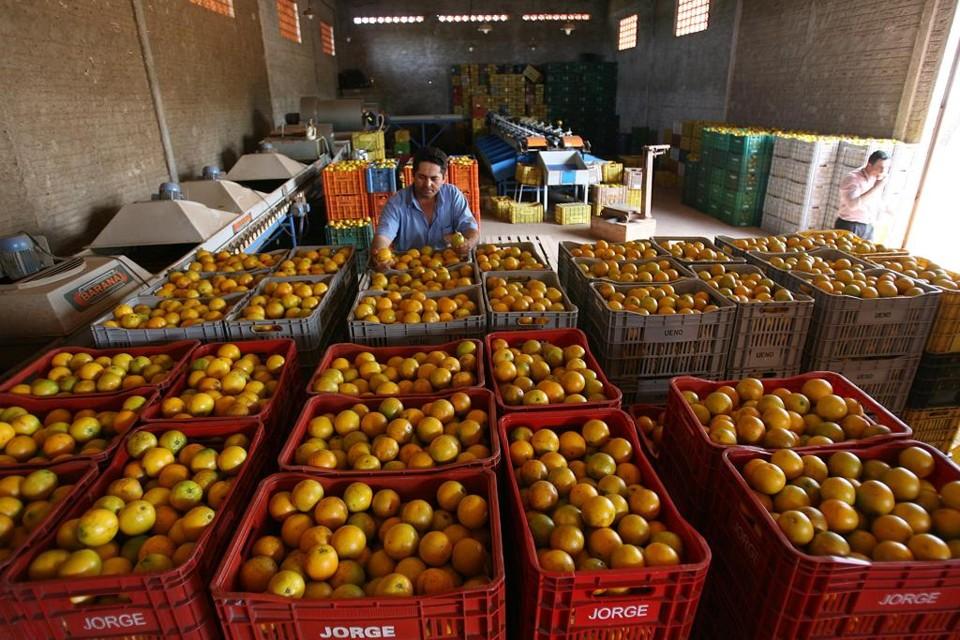
\includegraphics[width=9.5cm, height=5.5cm, keepaspectratio]{laranja_lotes.jpg} \\
    \small \textbf{Figura 2.1:} Colheitas e atividades operacionais coordenadas por colaboradores nas fazendas da cooperativa.
\end{center}

\vspace{0.3cm}
\begin{center}
    \textbf{Modelo Conceitual (Diagrama Entidade-Relacionamento)} \\[0.2cm]
    \begin{tikzpicture}[node distance=1.5cm, >=stealth, thick, scale=0.9, every node/.style={transform shape}]
        \node[block] (func) {Funcionario};
        \node[diamond_node, right=2.2cm of func] (alocado) {Alocado};
        \node[block, right=2.2cm of alocado] (fazenda) {Fazenda};
        
        \path[line] (func) -- (alocado);
        \path[line] (alocado) -- (fazenda);
        
        % Atributos Funcionario
        \node[attribute, above left=1cm and 0.4cm of func] (id_func) {\underline{id\_func}};
        \node[attribute, left=1.2cm of func] (nome) {nome};
        \node[attribute, below left=1cm and 0.4cm of func] (cargo) {cargo};
        \node[attribute, above=0.8cm of func] (cpf) {cpf};
        
        \path[line] (func) -- (id_func);
        \path[line] (func) -- (nome);
        \path[line] (func) -- (cargo);
        \path[line] (func) -- (cpf);
        
        % Atributos Fazenda
        \node[attribute, above right=1cm and 0.4cm of fazenda] (id_faz) {\underline{id\_fazenda}};
        \node[attribute, right=1.2cm of fazenda] (nome_faz) {nome\_fazenda};
        \node[attribute, below right=1cm and 0.4cm of fazenda] (prod) {produtor};
        \node[attribute, above=0.8cm of fazenda] (mun) {municipio};
        
        \path[line] (fazenda) -- (id_faz);
        \path[line] (fazenda) -- (nome_faz);
        \path[line] (fazenda) -- (prod);
        \path[line] (fazenda) -- (mun);
        
        % Atributo no Relacionamento
        \node[attribute, below=0.8cm of alocado] (dt_aloc) {data\_alocacao};
        \path[line] (alocado) -- (dt_aloc);
        
        % Cardinalidades
        \node[above, font=\small\bfseries] at ($(func.east)!0.3!(alocado.west)$) {N};
        \node[above, font=\small\bfseries] at ($(fazenda.west)!0.3!(alocado.east)$) {N};
    \end{tikzpicture}
\end{center}

\begin{center}
    \textbf{Modelo Lógico (Relacional)} \\[0.2cm]
    \begin{tikzpicture}[node distance=1.5cm, >=stealth, thick]
        \node[table_block] (func_tbl) at (0,0) {
            \textbf{tbFuncionario} \\
            \rule{4.1cm}{0.4pt} \\
            \underline{id\_func} (PK) \\
            nome: TEXT \\
            cargo: TEXT \\
            cpf: TEXT
        };
        
        \node[table_block] (comp_tbl) at (6.2,0) {
            \textbf{tbFuncionarioFazenda} \\
            \rule{4.1cm}{0.4pt} \\
            \underline{id\_func} (PK, FK) \\
            \underline{id\_fazenda} (PK, FK) \\
            data\_alocacao: TEXT
        };
        
        \node[table_block] (faz_tbl) at (12.4,0) {
            \textbf{tbFazenda} \\
            \rule{4.1cm}{0.4pt} \\
            \underline{id\_fazenda} (PK) \\
            nome\_fazenda: TEXT \\
            produtor: TEXT \\
            municipio: TEXT
        };
        
        \draw[->, color=forestgreen, ultra thick] (comp_tbl.west) -- (func_tbl.east) 
            node[midway, above, font=\scriptsize\bfseries, text=forestgreen] {FK: id\_func};
        \draw[->, color=forestgreen, ultra thick] (comp_tbl.east) -- (faz_tbl.west) 
            node[midway, above, font=\scriptsize\bfseries, text=forestgreen] {FK: id\_fazenda};
    \end{tikzpicture}
\end{center}

\begin{center}
    \textbf{Protótipos Wireframe do CRUD Completo (Visualização Individual - Um por Linha)} \\[0.3cm]
    
    % --- TELA READ (R) ---
    \resizebox{14cm}{!}{%
    \begin{tikzpicture}[scale=0.95, every node/.style={transform shape}]
      \node[screen] (r_scr) at (0,0) {};
      \node[screen_title, below=0.1cm of r_scr.north] (r_title) {Alocação de Funcionários - Tabela (R)};
      \node[btn, below=0.2cm of r_title, xshift=-2.8cm] (btn_novo) {+ Nova Alocação};
      
      % Table Frame / Grid
      \node[draw=gray!30, fill=white, minimum width=8.1cm, minimum height=3.0cm, below=0.8cm of r_title] (tbl_grid) {};
      
      % Table Header
      \node[draw=forestgreen!20, fill=forestgreen!5, minimum width=8.1cm, minimum height=0.6cm, below=0.8cm of r_title] (th) {};
      \node at (th.west) [anchor=west, xshift=0.2cm, font=\tiny\bfseries\sffamily] {Funcionário \hspace{0.5cm} Fazenda \hspace{0.5cm} Cargo \hspace{0.8cm} Alocação \hspace{0.3cm} Ações};
      
      % Row 1
      \node[draw=gray!10, fill=white, minimum width=8.1cm, minimum height=0.6cm, below=0.0cm of th] (r1) {};
      \node at (r1.west) [anchor=west, xshift=0.2cm, font=\tiny\sffamily] {João Silva \hspace{0.6cm} Recanto \hspace{0.5cm} Tratorista \hspace{0.5cm} 18/05/26 \hspace{0.3cm} [Edit] [X]};
      
      % Row 2
      \node[draw=gray!10, fill=gray!2, minimum width=8.1cm, minimum height=0.6cm, below=0.0cm of r1] (r2) {};
      \node at (r2.west) [anchor=west, xshift=0.2cm, font=\tiny\sffamily] {Maria Souza \hspace{0.4cm} Recanto \hspace{0.5cm} Agrônoma \hspace{0.5cm} 18/05/26 \hspace{0.3cm} [Edit] [X]};
      
      % Row 3
      \node[draw=gray!10, fill=white, minimum width=8.1cm, minimum height=0.6cm, below=0.0cm of r2] (r3) {};
      \node at (r3.west) [anchor=west, xshift=0.2cm, font=\tiny\sffamily] {Pedro Alves \hspace{0.4cm} Sol Nas. \hspace{0.4cm} Operador \hspace{0.6cm} 18/05/26 \hspace{0.3cm} [Edit] [X]};
      
      % Paginação
      \node[draw, fill=forestgreen, text=white, circle, inner sep=2pt, font=\scriptsize, above=0.4cm of r_scr.south, xshift=-1.2cm] (p1) {1};
      \node[draw, circle, inner sep=2pt, font=\scriptsize, right=0.25cm of p1] (p2) {2};
      \node[draw, circle, inner sep=2pt, font=\scriptsize, right=0.25cm of p2] (p3) {3};
      \node[font=\scriptsize, right=0.25cm of p3] (next) {Próxima >>};
    \end{tikzpicture}%
    }
    \\[0.5cm]
    
    % --- TELA CREATE/UPDATE (C/U) ---
    \resizebox{11cm}{!}{%
    \begin{tikzpicture}[scale=0.95, every node/.style={transform shape}]
      \node[screen] (cu_scr) at (0,0) {};
      \node[screen_title] at (0, 3.1) {Alocação de Funcionário - Cadastro (C/U)};
      
      \node[font=\footnotesize\bfseries\sffamily, anchor=west] at (-3.75, 2.2) {Selecione o Funcionário (FK id\_func):};
      \node[input_field, anchor=center] at (0, 1.78) {1001 - João Silva};
      
      \node[font=\footnotesize\bfseries\sffamily, anchor=west] at (-3.75, 1.1) {Selecione a Fazenda (FK id\_fazenda):};
      \node[input_field, anchor=center] at (0, 0.68) {2 - Fazenda Recanto};
      
      \node[font=\footnotesize\bfseries\sffamily, anchor=west] at (-3.75, 0.0) {Data da Alocação:};
      \node[input_field, anchor=center] at (0, -0.42) {18/05/2026};
      
      \node[btn, anchor=center, minimum width=2.5cm, minimum height=0.6cm] at (-1.5, -2.8) {Salvar Alocação};
      \node[btn_danger, anchor=center, minimum width=2.0cm, minimum height=0.6cm] at (1.3, -2.8) {Cancelar};
    \end{tikzpicture}%
    }
    \\[0.5cm]
    
    % --- TELA DELETE (D) ---
    \resizebox{11cm}{!}{%
    \begin{tikzpicture}[scale=0.95, every node/.style={transform shape}]
      \node[screen] (d_scr) at (0,0) {};
      \node[screen_title, below=0.1cm of d_scr.north] (d_title) {Alocação de Funcionário - Desvincular (D)};
      
      \node[draw=red!30, fill=red!5, rounded corners=6pt, minimum width=8.1cm, minimum height=3.5cm, below=0.8cm of d_title] (alert_box) {};
      \node[text=red, font=\footnotesize\bfseries\sffamily, align=center, yshift=1.2cm] at (alert_box) {CONFIRMAÇÃO DE DESVÍNCULO};
      \node[font=\footnotesize\sffamily, align=center, text width=7.5cm, yshift=0.3cm] at (alert_box) {Deseja realmente desassociar \textbf{João Silva} da \textbf{Fazenda Recanto}?};
      \node[font=\tiny\sffamily, align=center, text=red, text width=7.5cm, yshift=-0.6cm] at (alert_box) {\textbf{Aviso de Integridade:} Esta ação remove apenas a alocação. O funcionário e a fazenda continuarão cadastrados de forma independente no sistema!};
      
      \node[btn_danger, above=0.35cm of d_scr.south, xshift=-1.35cm, minimum width=2.2cm, minimum height=0.5cm] (btn_conf_del) {Desvincular};
      \node[btn, right=0.5cm of btn_conf_del, minimum width=2.2cm, minimum height=0.5cm] (btn_voltar) {Cancelar};
    \end{tikzpicture}%
    }
\end{center}

\vspace{0.4cm}

\begin{enumerate}[label=\textbf{\alph*)}]
    \item Desenvolva a estrutura DDL completa para criar as tabelas \textbf{tbFuncionario}, \textbf{tbFazenda} e a tabela associativa de junção Many-to-Many (N:N) chamada \textbf{tbFuncionarioFazenda}. Lembre-se de configurar a chave primária composta e as chaves estrangeiras na tabela de junção.
    \resposta{5cm}
    
    \item Escreva a consulta SQL necessária para renderizar a \textbf{Página 1} e a \textbf{Página 3} dessa listagem associativa (\textbf{tbFuncionarioFazenda}), trazendo os nomes dos funcionários, os nomes das fazendas e seus cargos correspondentes através de junções (`JOIN`). Os registros devem ser listados em ordem alfabética por nome de funcionário. O tamanho da página é de 15 registros.
    \resposta{4cm}

    \item Se representarmos a página desejada como uma variável $N$ em uma linguagem de programação (ex: Python), deduza uma consulta SQL contendo a expressão de cálculo dinâmico das cláusulas `LIMIT` e `OFFSET` para retornar a \textbf{Página $N$}.
    \resposta{2.5cm}

    \item \textbf{Edição (Update):} Devido a uma alteração na escala de trabalho itinerante, o cargo atribuído a João Silva (\texttt{id\_func = 1001}) na Fazenda Recanto (\texttt{id\_fazenda = 2}) mudou de \texttt{'Auxiliar'} para \texttt{'Tratorista'}. Escreva a instrução SQL para corrigir esta função na tabela associativa.
    \resposta{2.5cm}

    \item \textbf{Regra de Negócio (Integridade Referencial):} Em um relacionamento Many-to-Many (N:N) implementado via tabela de junção, analise o impacto das exclusões nas tabelas principais:
    \begin{enumerate}[label=\arabic*.]
        \item Caso um funcionário seja desligado (deletado) ou uma fazenda seja vendida (deletada) do sistema da cooperativa, o que deve ocorrer automaticamente com os registros correspondentes na tabela associativa \textbf{tbFuncionarioFazenda} para manter a consistência física? Identifique qual cláusula/ação de integridade garante esse comportamento.
        \item Escreva a DDL das restrições de chave estrangeira (FK) na tabela associativa \textbf{tbFuncionarioFazenda} que implementam esse comportamento de forma implícita.
    \end{enumerate}
    \resposta{4.5cm}
\end{enumerate}

% ------------------------------------------------
% EXERCÍCIO 3
% ------------------------------------------------
\section*{Exercício 3}

\textbf{Contexto:} Em um sistema de monitoramento pecuário de alta precisão (Pecuária 4.0), cada bovino de elite monitorado é equipado com um colar sensor inteligente (GPS + acelerômetro para monitorar saúde e pastejo). Para evitar duplicidade de dados e leituras cruzadas, a regra de negócio determina uma relação estrita de 1 para 1: cada boi pode usar no máximo um colar ativo por vez, e cada colar sensor só pode estar associado a um único bovino. O aplicativo móvel do peão permite gerenciar e listar o emparelhamento ativo de colares e bois, exibindo os dados paginados.

\begin{center}
    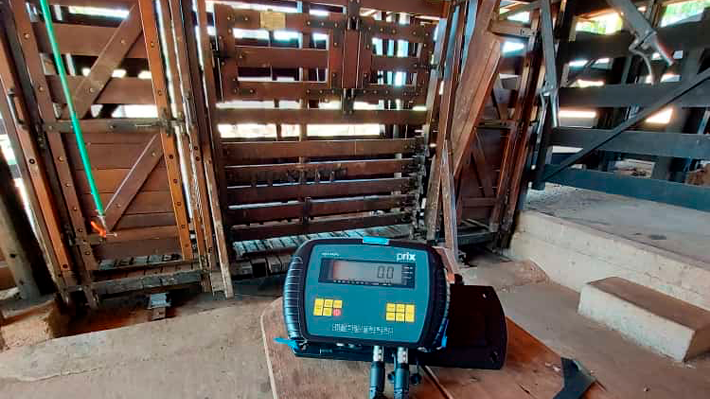
\includegraphics[width=9.5cm, height=5.5cm, keepaspectratio]{pesagem_bovino.png} \\
    \small \textbf{Figura 3.1:} Monitoramento individual de bovinos equipados com colares coletores de dados e localização.
\end{center}

\vspace{0.3cm}
\begin{center}
    \textbf{Modelo Conceitual (Diagrama Entidade-Relacionamento)} \\[0.2cm]
    \begin{tikzpicture}[node distance=1.5cm, >=stealth, thick, scale=0.9, every node/.style={transform shape}]
        \node[block] (boi) {Bovino};
        \node[diamond_node, right=2.2cm of boi] (equipado) {Equipado};
        \node[block, right=2.2cm of equipado] (colar) {Colar};
        
        \path[line] (boi) -- (equipado);
        \path[line] (equipado) -- (colar);
        
        % Atributos Bovino
        \node[attribute, above left=1cm and 0.4cm of boi] (id_boi) {\underline{id\_boi}};
        \node[attribute, left=1.2cm of boi] (brinco) {brinco\_rfid};
        \node[attribute, below left=1cm and 0.4cm of boi] (peso) {peso\_estimado};
        \node[attribute, above=0.8cm of boi] (raca) {raca};
        
        \path[line] (boi) -- (id_boi);
        \path[line] (boi) -- (brinco);
        \path[line] (boi) -- (peso);
        \path[line] (boi) -- (raca);
        
        % Atributos Colar
        \node[attribute, above right=1cm and 0.4cm of colar] (id_colar) {\underline{id\_colar}};
        \node[attribute, right=1.2cm of colar] (num_serie) {numero\_serie};
        \node[attribute, below right=1cm and 0.4cm of colar] (bat) {bateria\_percent};
        \node[attribute, above=0.8cm of colar] (status) {status};
        
        \path[line] (colar) -- (id_colar);
        \path[line] (colar) -- (num_serie);
        \path[line] (colar) -- (bat);
        \path[line] (colar) -- (status);
        
        % Cardinalidades
        \node[above, font=\small\bfseries] at ($(boi.east)!0.3!(equipado.west)$) {1};
        \node[above, font=\small\bfseries] at ($(colar.west)!0.3!(equipado.east)$) {1};
    \end{tikzpicture}
\end{center}

\begin{center}
    \textbf{Modelo Lógico (Relacional)} \\[0.2cm]
    \begin{tikzpicture}[node distance=1.5cm, >=stealth, thick]
        \node[table_block] (colar_tbl) at (0,0) {
            \textbf{tbColar} \\
            \rule{4.1cm}{0.4pt} \\
            \underline{id\_colar} (PK) \\
            numero\_serie: TEXT \\
            bateria\_percent: INTEGER \\
            status: TEXT
        };
        
        \node[table_block] (boi_tbl) at (12,0) {
            \textbf{tbBovino} \\
            \rule{4.1cm}{0.4pt} \\
            \underline{id\_boi} (PK) \\
            brinco\_rfid: TEXT \\
            peso\_estimado: REAL \\
            raca: TEXT \\
            id\_colar (FK, UNIQUE)
        };
        \draw[->, color=forestgreen, ultra thick] (boi_tbl.west) -- (colar_tbl.east) 
            node[midway, above, font=\scriptsize\bfseries, text=forestgreen] {FK: id\_colar $\rightarrow$ tbColar(id\_colar)};
    \end{tikzpicture}
\end{center}

\begin{center}
    \textbf{Protótipos Wireframe do CRUD Completo (Visualização Individual - Um por Linha)} \\[0.3cm]
    
    % --- TELA READ (R) ---
    \resizebox{16.5cm}{!}{%
    \begin{tikzpicture}[scale=0.95, every node/.style={transform shape}]
      \node[screen] (r_scr) at (0,0) {};
      \node[screen_title, below=0.1cm of r_scr.north] (r_title) {RFID Pesagens - Listagem em Acordeão (R)};
      \node[btn, below=0.2cm of r_title, xshift=-2.8cm] (btn_novo) {+ Novo Vínculo};
      
      % Accordion Item 1 (EXPANDED)
      \node[draw=forestgreen!30, fill=green!2, rounded corners=4pt, minimum width=8.1cm, minimum height=1.7cm, below=0.8cm of r_title] (acc1) {};
      \node at (acc1.north west) [anchor=north west, xshift=0.2cm, yshift=-0.15cm, font=\footnotesize\bfseries\sffamily] {\textcolor{forestgreen}{[-] Brinco: BR2026-X (Nelore) $\blacktriangledown$}};
      \node at (acc1.west) [anchor=west, xshift=0.2cm, yshift=-0.2cm, font=\tiny\sffamily, align=left] {
          Colar Pareado: \textbf{\#COL-7729} \hspace{0.5cm} Bateria: \textbf{85\%} \\
          Status GPS: Monitoramento Ativo \hspace{0.5cm} Peso Est: 420.5 kg
      };
      \node[btn, right=0.2cm of acc1.east, anchor=east, xshift=-1.1cm, yshift=0.4cm] (edit1) {Editar};
      \node[btn_danger, right=0.2cm of acc1.east, anchor=east, xshift=-0.2cm, yshift=0.4cm] (del1) {Excluir};
      
      % Accordion Item 2 (COLLAPSED)
      \node[draw=gray!30, fill=white, rounded corners=4pt, minimum width=8.1cm, minimum height=0.7cm, below=0.15cm of acc1] (acc2) {};
      \node at (acc2.west) [anchor=west, xshift=0.2cm, font=\footnotesize\bfseries\sffamily] {[+] Brinco: BR2026-Y (Garrote) $\blacktriangleright$};
      
      % Accordion Item 3 (COLLAPSED)
      \node[draw=gray!30, fill=white, rounded corners=4pt, minimum width=8.1cm, minimum height=0.7cm, below=0.15cm of acc2] (acc3) {};
      \node at (acc3.west) [anchor=west, xshift=0.2cm, font=\footnotesize\bfseries\sffamily] {[+] Brinco: BR2026-Z (Novilha) $\blacktriangleright$};
      
      % Paginação
      \node[draw, fill=forestgreen, text=white, circle, inner sep=2pt, font=\scriptsize, above=0.4cm of r_scr.south, xshift=-1.2cm] (p1) {1};
      \node[draw, circle, inner sep=2pt, font=\scriptsize, right=0.25cm of p1] (p2) {2};
      \node[draw, circle, inner sep=2pt, font=\scriptsize, right=0.25cm of p2] (p3) {3};
      \node[font=\scriptsize, right=0.25cm of p3] (next) {Próxima >>};
    \end{tikzpicture}%
    }
    \\[0.5cm]
    
    % --- TELA CREATE/UPDATE (C/U) ---
    \resizebox{11cm}{!}{%
    \begin{tikzpicture}[scale=0.95, every node/.style={transform shape}]
      \node[screen] (cu_scr) at (0,0) {};
      \node[screen_title] at (0, 3.1) {Emparelhamento - Cadastro (C/U)};
      
      \node[font=\footnotesize\bfseries\sffamily, anchor=west] at (-3.75, 2.0) {Identificação do Brinco RFID:};
      \node[input_field, anchor=center] at (0, 1.55) {BR2026-X};
      
      \node[font=\footnotesize\bfseries\sffamily, anchor=west] at (-3.75, 0.85) {Selecione o Colar (FK id\_colar):};
      \node[input_field, anchor=center] at (0, 0.4) {55 - Serie COL-7729};
      
      \node[font=\footnotesize\bfseries\sffamily, anchor=west] at (-3.75, -0.3) {Status do Dispositivo:};
      \node[input_field, anchor=center] at (0, -0.75) {Monitoramento Ativo};
      
      \node[btn, anchor=center, minimum width=2.5cm, minimum height=0.6cm] at (-1.5, -2.8) {Salvar Emparelhamento};
      \node[btn_danger, anchor=center, minimum width=2.0cm, minimum height=0.6cm] at (1.3, -2.8) {Cancelar};
    \end{tikzpicture}
    }
    \\[0.5cm]
    
    % --- TELA DELETE (D) ---
    \resizebox{11cm}{!}{%
    \begin{tikzpicture}[scale=0.95, every node/.style={transform shape}]
      \node[screen] (d_scr) at (0,0) {};
      \node[screen_title, below=0.1cm of d_scr.north] (d_title) {Emparelhamento - Desvincular (D)};
      
      \node[draw=red!30, fill=red!5, rounded corners=6pt, minimum width=8.1cm, minimum height=3.5cm, below=0.8cm of d_title] (alert_box) {};
      \node[text=red, font=\footnotesize\bfseries\sffamily, align=center, yshift=1.2cm] at (alert_box) {CONFIRMAÇÃO DE DESVÍNCULO};
      \node[font=\footnotesize\sffamily, align=center, text width=7.5cm, yshift=0.3cm] at (alert_box) {Deseja realmente desvincular o \textbf{Colar \#COL-7729} do bovino \textbf{BR2026-X}?};
      \node[font=\tiny\sffamily, align=center, text=red, text width=7.5cm, yshift=-0.6cm] at (alert_box) {\textbf{Aviso de Integridade:} Desemparelhar desassociará o colar do boi, mas manterá os registros originais intactos nas tabelas principais.};
      
      \node[btn_danger, above=0.35cm of d_scr.south, xshift=-1.35cm, minimum width=2.2cm, minimum height=0.5cm] (btn_conf_del) {Desvincular};
      \node[btn, right=0.5cm of btn_conf_del, minimum width=2.2cm, minimum height=0.5cm] (btn_voltar) {Cancelar};
    \end{tikzpicture}%
    }
\end{center}

\vspace{0.4cm}

\begin{enumerate}[label=\textbf{\alph*)}]
    \item Escreva a definição DDL completa para as tabelas \textbf{tbColar} e \textbf{tbBovino}, configurando corretamente a chave estrangeira e restrições necessárias para garantir a integridade de um relacionamento de 1 para 1 (1:1).
    \resposta{5cm}
    
    \item Escreva a consulta SQL com junção (`JOIN`) para listar o histórico de todos os emparelhamentos ativos de bovinos e colares, trazendo o brinco rfid do animal, a raça, o número de série do colar e a bateria correspondente, ordenados de forma crescente pelo brinco. O tamanho da página é de 8 registros.
    \resposta{4cm}

    \item Ao realizar uma exportação manual do histórico de emparelhamentos, o sistema saltou os primeiros 40 registros. A qual \textbf{página} do aplicativo móvel essa exportação corresponde? Demonstre e escreva a consulta SQL correspondente para retornar essas linhas puladas.
    \resposta{2.5cm}

    \item \textbf{Edição (Update):} Devido a uma necessidade de manutenção do hardware, o Colar \#COL-7729 (\texttt{id\_colar = 55}) atribuído ao bovino com brinco \texttt{'BR2026-X'} (\texttt{id\_boi = 102}) foi substituído pelo Colar \#COL-8000 (\texttt{id\_colar = 60}). Escreva a consulta SQL para realizar essa alteração na tabela correspondente.
    \resposta{2.5cm}

    \item \textbf{Regra de Negócio (Integridade Referencial):} Em um relacionamento de 1 para 1 (1:1) com chave estrangeira opcional em uma das entidades pais:
    \begin{enumerate}[label=\arabic*.]
        \item Se um colar sensor for danificado e deletado do inventário (\texttt{tbColar}), o que deve ocorrer automaticamente com o campo de referência do bovino associado em \texttt{tbBovino} para que o animal continue cadastrado no sistema, porém sem colar? Identifique qual regra/ação de integridade referencial implementa essa restrição de forma automática.
        \item Escreva a DDL de restrição de chave estrangeira (FK) na tabela \textbf{tbBovino} que ative esse comportamento.
    \end{enumerate}
    \resposta{4.5cm}
\end{enumerate}

% ------------------------------------------------
% EXERCÍCIO 4
% ------------------------------------------------
\section*{Exercício 4}

\textbf{Contexto:} Para atender às exigências de exportação e conformidade ecológica, uma grande trading de grãos audita o registro de aplicações fitossanitárias em lavouras de algodão. Como a tabela de pulverizações possui milhares de registros, os auditores analisam as aplicações em páginas de 12 registros. Esta consulta exige dados combinados da aplicação (produto, data, dosagem) e do respectivo talhão onde o produto foi pulverizado (código do talhão, cultura instalada).

\begin{center}
    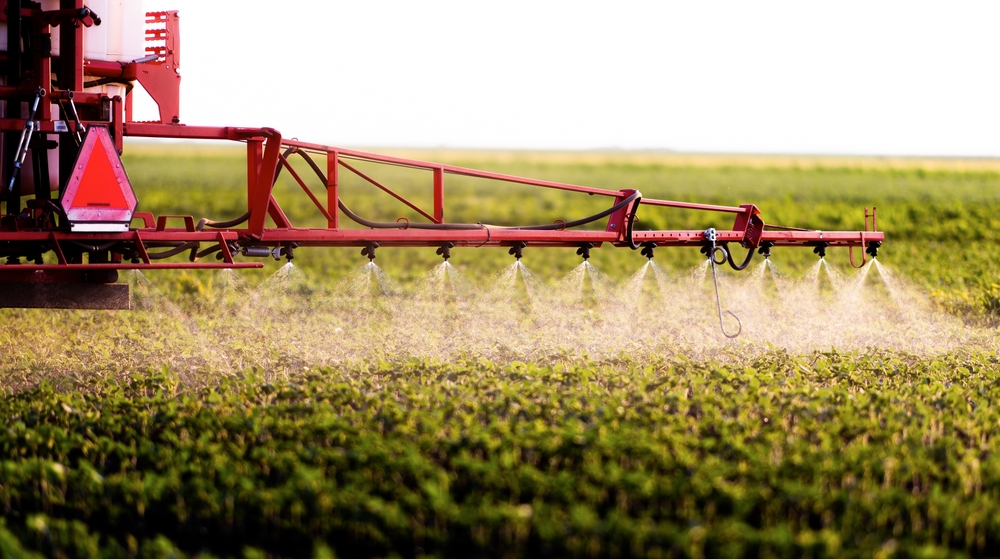
\includegraphics[width=6.8cm, height=4.8cm, keepaspectratio]{pulverizacao.jpg}
    \hspace{0.6cm}
    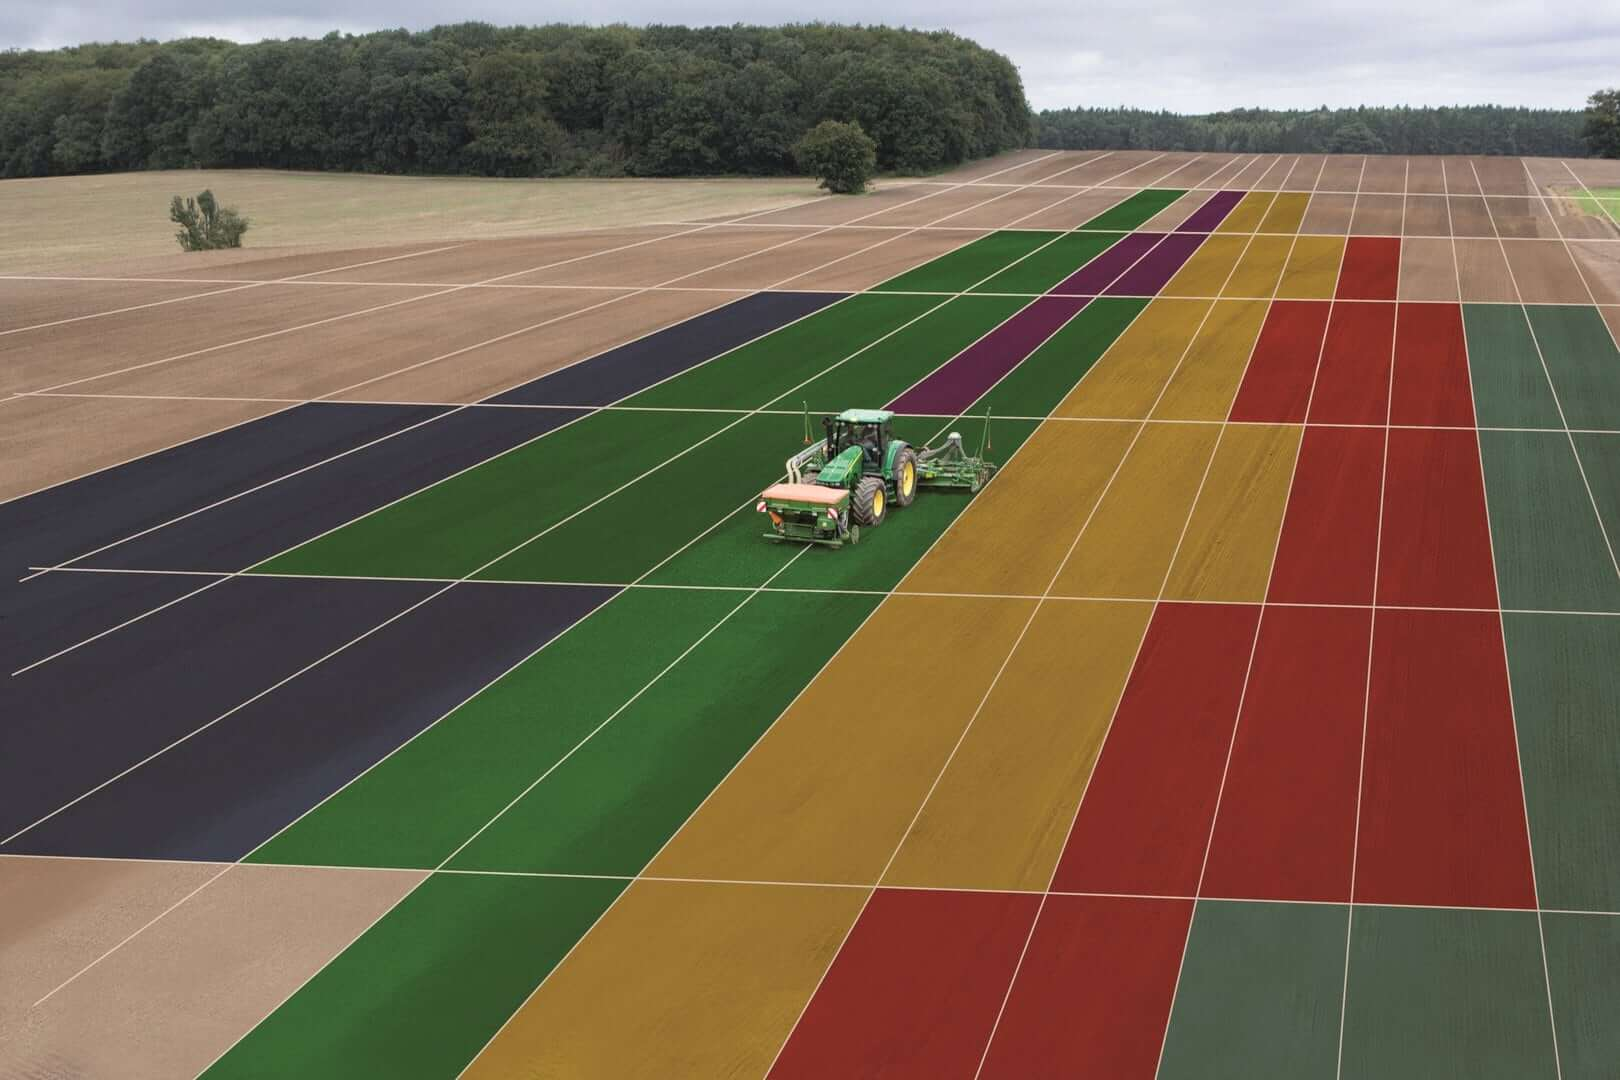
\includegraphics[width=6.8cm, height=4.8cm, keepaspectratio]{talhao.jpg} \\
    \small \textbf{Figura 4.1:} Processo de pulverização fitossanitária (esquerda) e visualização aérea dos talhões monitorados (direita).
\end{center}

\vspace{0.3cm}
\begin{center}
    \textbf{Modelo Conceitual (Diagrama Entidade-Relacionamento)} \\[0.2cm]
    \begin{tikzpicture}[node distance=1.5cm, >=stealth, thick, scale=0.9, every node/.style={transform shape}]
        \node[block] (talhao) {Talhao};
        \node[diamond_node, right=2.2cm of talhao] (recebe) {Recebe};
        \node[block, right=2.2cm of recebe] (pulv) {Aplicacao};
        
        \path[line] (talhao) -- (recebe);
        \path[line] (recebe) -- (pulv);
        
        % Atributos Talhao
        \node[attribute, above left=1cm and 0.4cm of talhao] (id_tal) {\underline{id\_talhao}};
        \node[attribute, left=1.2cm of talhao] (cod) {codigo\_talhao};
        \node[attribute, below left=1cm and 0.4cm of talhao] (area) {area\_ha};
        \node[attribute, above=0.8cm of talhao] (cult) {tipo\_cultura};
        
        \path[line] (talhao) -- (id_tal);
        \path[line] (talhao) -- (cod);
        \path[line] (talhao) -- (area);
        \path[line] (talhao) -- (cult);
        
        % Atributos Aplicacao
        \node[attribute, above right=1cm and 0.4cm of pulv] (id_pulv) {\underline{id\_pulv}};
        \node[attribute, right=1.2cm of pulv] (prod) {produto};
        \node[attribute, below right=1cm and 0.4cm of pulv] (dt) {data\_pulv};
        \node[attribute, above=0.8cm of pulv] (dose) {dosagem\_l\_ha};
        
        \path[line] (pulv) -- (id_pulv);
        \path[line] (pulv) -- (prod);
        \path[line] (pulv) -- (dt);
        \path[line] (pulv) -- (dose);
        
        % Cardinalidades
        \node[above, font=\small\bfseries] at ($(talhao.east)!0.3!(recebe.west)$) {1};
        \node[above, font=\small\bfseries] at ($(pulv.west)!0.3!(recebe.east)$) {N};
    \end{tikzpicture}
\end{center}

\begin{center}
    \textbf{Modelo Lógico (Relacional)} \\[0.4cm]
    \begin{tikzpicture}[node distance=5cm, >=stealth, thick]
        \node[table_block] (tal_tbl) at (0,0) {
            \textbf{tbTalhao} \\
            \rule{4.1cm}{0.4pt} \\
            \underline{id\_talhao} (PK) \\
            codigo\_talhao: TEXT \\
            area\_ha: REAL \\
            tipo\_cultura: TEXT
        };
        
        \node[table_block] (pulv_tbl) at (12,0) {
            \textbf{tbAplicacao} \\
            \rule{4.1cm}{0.4pt} \\
            \underline{id\_pulv} (PK) \\
            produto: TEXT \\
            data\_pulv: TEXT \\
            dosagem\_l\_ha: REAL \\
            id\_talhao (FK)
        };
        
        \draw[->, color=forestgreen, ultra thick] (pulv_tbl.west) -- (tal_tbl.east) 
            node[midway, above, font=\scriptsize\bfseries, text=forestgreen] {FK: id\_talhao $\rightarrow$ tbTalhao(id\_talhao)};
    \end{tikzpicture}
\end{center}

\begin{center}
    \textbf{Protótipos Wireframe do CRUD Completo (Visualização Individual - Um por Linha)} \\[0.3cm]
    
    % --- TELA READ (R) ---
    \resizebox{11cm}{!}{%
    \begin{tikzpicture}[scale=0.95, every node/.style={transform shape}]
      \node[screen] (r_scr) at (0,0) {};
      \node[screen_title, below=0.1cm of r_scr.north] (r_title) {Aplicações Fitossanitárias - Tabela (R)};
      \node[btn, below=0.2cm of r_title, xshift=-2.8cm] (btn_novo) {+ Nova Aplicação};
      
      % Table Frame / Grid
      \node[draw=gray!30, fill=white, minimum width=8.1cm, minimum height=3.0cm, below=0.8cm of r_title] (tbl_grid) {};
      
      % Table Header
      \node[draw=forestgreen!20, fill=forestgreen!5, minimum width=8.1cm, minimum height=0.6cm, below=0.8cm of r_title] (th) {};
      \node at (th.west) [anchor=west, xshift=0.15cm, font=\tiny\bfseries\sffamily] {Talhão \hspace{0.4cm} Cultura \hspace{0.4cm} Produto \hspace{0.5cm} Dosagem \hspace{0.4cm} Ações};
      
      % Row 1
      \node[draw=gray!10, fill=white, minimum width=8.1cm, minimum height=0.6cm, below=0.0cm of th] (r1) {};
      \node at (r1.west) [anchor=west, xshift=0.15cm, font=\tiny\sffamily] {T03 \hspace{0.6cm} Algodão \hspace{0.3cm} Glypho \hspace{0.5cm} 2.5 L/ha \hspace{0.4cm} [Editar] [X]};
      
      % Row 2
      \node[draw=gray!10, fill=gray!2, minimum width=8.1cm, minimum height=0.6cm, below=0.0cm of r1] (r2) {};
      \node at (r2.west) [anchor=west, xshift=0.15cm, font=\tiny\sffamily] {T01 \hspace{0.6cm} Soja \hspace{0.7cm} Fungic \hspace{0.5cm} 1.2 L/ha \hspace{0.4cm} [Editar] [X]};
      
      % Row 3
      \node[draw=gray!10, fill=white, minimum width=8.1cm, minimum height=0.6cm, below=0.0cm of r2] (r3) {};
      \node at (r3.west) [anchor=west, xshift=0.15cm, font=\tiny\sffamily] {T04 \hspace{0.6cm} Milho \hspace{0.6cm} Insetic \hspace{0.5cm} 0.8 L/ha \hspace{0.4cm} [Editar] [X]};
      
      % Paginação
      \node[draw, fill=forestgreen, text=white, circle, inner sep=2pt, font=\scriptsize, above=0.4cm of r_scr.south, xshift=-1.2cm] (p1) {1};
      \node[draw, circle, inner sep=2pt, font=\scriptsize, right=0.25cm of p1] (p2) {2};
      \node[draw, circle, inner sep=2pt, font=\scriptsize, right=0.25cm of p2] (p3) {3};
      \node[font=\scriptsize, right=0.25cm of p3] (next) {Próxima >>};
    \end{tikzpicture}%
    }
    \\[0.5cm]
    
    % --- TELA CREATE/UPDATE (C/U) ---
    \resizebox{11cm}{!}{%
    \begin{tikzpicture}[scale=0.95, every node/.style={transform shape}]
      \node[screen] (cu_scr) at (0,0) {};
      \node[screen_title] at (0, 3.1) {Aplicação - Formulário (C/U)};
      
      \node[font=\footnotesize\bfseries\sffamily, anchor=west] at (-3.75, 2.2) {Defensivo / Produto:};
      \node[input_field, anchor=center] at (0, 1.78) {Glifosato Herbicida};
      
      \node[font=\footnotesize\bfseries\sffamily, anchor=west] at (-3.75, 1.1) {Dosagem Aplicada (L/ha):};
      \node[input_field, anchor=center] at (0, 0.68) {2.5};
      
      \node[font=\footnotesize\bfseries\sffamily, anchor=west] at (-3.75, 0.0) {Data da Aplicação:};
      \node[input_field, anchor=center] at (0, -0.42) {18/05/2026};
      
      \node[font=\footnotesize\bfseries\sffamily, anchor=west] at (-3.75, -1.1) {Talhão Destinatário (FK):};
      \node[input_field, anchor=center] at (0, -1.52) {3 - Talhão Oeste};
      
      \node[btn, anchor=center, minimum width=2.5cm, minimum height=0.6cm] at (-1.5, -2.8) {Salvar Registro};
      \node[btn_danger, anchor=center, minimum width=2.0cm, minimum height=0.6cm] at (1.3, -2.8) {Cancelar};
    \end{tikzpicture}%
    }
    \\[0.5cm]
    
    % --- TELA DELETE (D) ---
    \resizebox{11cm}{!}{%
    \begin{tikzpicture}[scale=0.95, every node/.style={transform shape}]
      \node[screen] (d_scr) at (0,0) {};
      \node[screen_title, below=0.1cm of d_scr.north] (d_title) {Aplicação - Excluir Registro (D)};
      
      \node[draw=red!30, fill=red!5, rounded corners=6pt, minimum width=8.1cm, minimum height=3.5cm, below=0.8cm of d_title] (alert_box) {};
      \node[text=red, font=\footnotesize\bfseries\sffamily, align=center, yshift=1.2cm] at (alert_box) {CONFIRMAÇÃO DE EXCLUSÃO};
      \node[font=\footnotesize\sffamily, align=center, text width=7.5cm, yshift=0.3cm] at (alert_box) {Deseja realmente excluir a aplicação do produto \textbf{Glifosato}?};
      
      \node[btn_danger, above=0.35cm of d_scr.south, xshift=-1.35cm, minimum width=2.2cm, minimum height=0.5cm] (btn_conf_del) {Sim, Excluir};
      \node[btn, right=0.5cm of btn_conf_del, minimum width=2.2cm, minimum height=0.5cm] (btn_voltar) {Cancelar};
    \end{tikzpicture}%
    }
\end{center}

\vspace{0.4cm}

\begin{enumerate}[label=\textbf{\alph*)}]
    \item Declare o script DDL para criar as tabelas \textbf{tbTalhao} e \textbf{tbAplicacao}, definindo integridade relacional.
    \resposta{5cm}
    
    \item Para obter a lista completa consolidada, é necessária uma junção de dados (`JOIN`). Escreva a consulta SQL para retornar a \textbf{Página 1} e a \textbf{Página 2} da auditoria, exibindo: \texttt{codigo\_talhao}, \texttt{tipo\_cultura}, \texttt{produto}, \texttt{data\_pulv} e \texttt{dosagem\_l\_ha}. Os registros devem ser listados em ordem cronológica reversa (pulverizações mais recentes no início). Tamanho da página: 12 registros.
    \resposta{4cm}

    \item Qual é a consequência técnica direta se omitirmos o \textbf{ORDER BY} in uma consulta paginada em um banco de dados real sujeito a inserções frequentes de dados? Explique se existe o risco de registros aparecerem duplicados em páginas diferentes ou não aparecerem na navegação.
    \resposta{2.5cm}

    \item \textbf{Edição (Update):} O Talhão Oeste (\texttt{id\_talhao = 3}) foi expandido e sua área aumentou de \texttt{45.2} hectares para \texttt{50.0} hectares, e a cultura ativa passou de \texttt{'Algodão'} para \texttt{'Milho Safrinha'}. Escreva a instrução SQL para atualizar este talhão.
    \resposta{2.5cm}

    \item \textbf{Exclusão (Delete):} Uma aplicação de \texttt{'Fungicida'} no dia 18/05 no Talhão Oeste (\texttt{id\_pulv = 704}) foi cancelada. Escreva o comando SQL para excluir esta pulverização e explique a diferença regulatória/referencial entre deletar uma aplicação versus remover o talhão inteiro do sistema.
    \resposta{3.5cm}
\end{enumerate}
% ------------------------------------------------
% EXERCÍCIO 5
% ------------------------------------------------
\section*{Exercício 5}

\textbf{Contexto:} Uma universidade gerencia o empréstimo de equipamentos de laboratório para professores e pesquisadores. Cada equipamento pode ser emprestado a um responsável, mas também pode ficar disponível no estoque sem estar emprestado. Quando um professor deixa a universidade, seus empréstimos ativos devem ser cancelados (os equipamentos retornam ao estoque), mas o registro do empréstimo deve ser mantido para histórico. Além disso, se o código de identificação de um equipamento for atualizado no sistema, todos os registros de empréstimo associados devem refletir essa mudança.

\begin{center}
    \textbf{Modelo Lógico (Relacional)} \\[0.2cm]
\begin{tikzpicture}[node distance=2cm, >=stealth, thick]

    % Linha superior
    \node[table_block] (prof_tbl) at (0,0) {
        \textbf{tbProfessor} \\
        \rule{3.5cm}{0.4pt} \\
        \underline{id\_prof} (PK) \\
        nome: TEXT \\
        departamento: TEXT \\
        email: TEXT
    };

    \node[table_block] (equip_tbl) at (6,0) {
        \textbf{tbEquipamento} \\
        \rule{3.5cm}{0.4pt} \\
        \underline{id\_equip} (PK) \\
        nome\_equip: TEXT \\
        numero\_serie: TEXT \\
        data\_aquisicao: TEXT
    };

    % Linha inferior
    \node[table_block] (emprest_tbl) at (3,-5) {
        \textbf{tbEmprestimo} \\
        \rule{3.5cm}{0.4pt} \\
        \underline{id\_emprest} (PK) \\
        data\_emprestimo: TEXT \\
        data\_devolucao: TEXT \\ 
        id\_prof (FK) \\
        id\_equip (FK)
    };

    % Relacionamentos
    \draw[->, color=forestgreen, ultra thick]
        (emprest_tbl.north west) -- (prof_tbl.south)
        node[midway, left, font=\scriptsize\bfseries, text=forestgreen]
        {FK: id\_prof};

    \draw[->, color=forestgreen, ultra thick]
        (emprest_tbl.north east) -- (equip_tbl.south)
        node[midway, right, font=\scriptsize\bfseries, text=forestgreen]
        {FK: id\_equip};

\end{tikzpicture}
\end{center} 

\begin{enumerate}[label=\textbf{\alph*)}]
    \item Escreva o script DDL completo para criar as três tabelas com as chaves primárias e estrangeiras apropriadas.
    \resposta{4cm}
    
    \item \textbf{Regra de Negócio (Integridade Referencial):} 
    \begin{enumerate}[label=\arabic*.]
        \item Quando um professor deixa a universidade e é removido do sistema, o que deve acontecer com os empréstimos ativos associados a esse professor para manter o histórico, mas liberar os equipamentos? Identifique a cláusula referencial adequada.
        \item Quando o código de identificação de um equipamento é atualizado no sistema, o que deve acontecer com as referências nesse código na tabela de empréstimos? Identifique a cláusula referencial adequada.
    \end{enumerate}
    \resposta{3cm}
    
    \item Escreva o script DDL das restrições de chave estrangeira na tabela \textbf{tbEmprestimo} que implementam o comportamento descrito no item (b).
    \resposta{3cm}
\end{enumerate}
% ------------------------------------------------
% EXERCÍCIO 6
% ------------------------------------------------
\section*{Exercício 6}

\textbf{Contexto:} Uma empresa possui um sistema de gestão de funcionários no qual cada funcionário pode possuir um supervisor direto, que também é um funcionário da própria empresa. Alguns funcionários, como diretores, não possuem supervisor. Quando um supervisor é removido do sistema, os funcionários subordinados não devem ser excluídos, mas devem ficar temporariamente sem supervisor até que outro seja designado. Além disso, caso o identificador de um supervisor seja alterado devido a uma migração de dados, todas as referências aos subordinados devem ser atualizadas automaticamente.

\begin{center}
    \textbf{Modelo Lógico (Relacional)} \\[0.2cm]

    \begin{tikzpicture}[node distance=2cm, >=stealth, thick]

        \node[table_block] (func_tbl) at (0,0) {
            \textbf{tbFuncionario} \\
            \rule{3.5cm}{0.4pt} \\
            \underline{id\_func} (PK) \\
            nome: TEXT \\
            cargo: TEXT \\
            salario: REAL \\
            id\_supervisor (FK)
        };

        % Auto-relacionamento
        \draw[->, color=forestgreen, ultra thick]
            (func_tbl.east) .. controls +(3,1.5) and +(3,-1.5) ..
            node[right, font=\scriptsize\bfseries, text=forestgreen]
            {FK: id\_supervisor}
            (func_tbl.east);

    \end{tikzpicture}
\end{center}

\begin{enumerate}[label=\textbf{\alph*)}]
    
    \item Escreva o script DDL completo para criar a tabela com a chave primária e a chave estrangeira autoreferenciada apropriada.
    \resposta{4cm}
    
    \item \textbf{Regra de Negócio (Integridade Referencial):}
    \begin{enumerate}[label=\arabic*.]
        \item Quando um supervisor é removido do sistema, o que deve acontecer com os funcionários subordinados para que permaneçam cadastrados, mas sem supervisor definido? Identifique a cláusula referencial adequada.
        
        \item Quando o identificador de um supervisor é alterado devido a uma migração de dados, o que deve acontecer com as referências aos subordinados? Identifique a cláusula referencial adequada.
    \end{enumerate}
    \resposta{3cm}
    
    \item Escreva o script DDL da restrição de chave estrangeira autoreferenciada na tabela \textbf{tbFuncionario} que implementa o comportamento descrito no item (b).
    \resposta{3cm}

\end{enumerate}

% ------------------------------------------------
% EXERCÍCIO 7
% ------------------------------------------------
\section*{Exercício 7}

\textbf{Contexto:} Uma editora gerencia o catálogo de livros e seus autores. Um livro pode ter múltiplos autores (coautoria), e um autor pode ter escrito múltiplos livros. Quando um livro é retirado de catálogo e excluído do sistema, todas as suas associações com autores devem ser removidas. Quando um autor deixa a editora e é excluído do sistema, todas as suas associações com livros devem ser mantidas para preservar o histórico das obras, mas o autor não deve mais estar associado a nenhum livro ativo.

\begin{center}
    \textbf{Modelo Lógico (Relacional)} \\[0.2cm]
    \begin{tikzpicture}[node distance=2.2cm, >=stealth, thick]

    % Linha superior
    \node[table_block] (livro_tbl) at (0,0) {
        \textbf{tbLivro} \\
        \rule{3.5cm}{0.4pt} \\
        \underline{id\_livro} (PK) \\
        titulo: TEXT \\
        ano\_publicacao: INTEGER \\
        editora: TEXT
    };

    \node[table_block] (autor_tbl) at (6,0) {
        \textbf{tbAutor} \\
        \rule{3.5cm}{0.4pt} \\
        \underline{id\_autor} (PK) \\
        nome: TEXT \\
        nacionalidade: TEXT \\
        data\_nasc: TEXT
    };

    % Linha inferior
    \node[table_block] (escrita_tbl) at (3,-5) {
        \textbf{tbAutorLivro} \\
        \rule{3.5cm}{0.4pt} \\
        \underline{id\_livro} (PK, FK) \\
        \underline{id\_autor} (PK, FK) \\
        ordem\_autoria: INTEGER
    };

    % Relacionamentos
    \draw[->, color=forestgreen, ultra thick]
        (escrita_tbl.north west) -- (livro_tbl.south)
        node[midway, left, font=\scriptsize\bfseries, text=forestgreen]
        {FK: id\_livro};

    \draw[->, color=forestgreen, ultra thick]
        (escrita_tbl.north east) -- (autor_tbl.south)
        node[midway, right, font=\scriptsize\bfseries, text=forestgreen]
        {FK: id\_autor};

\end{tikzpicture}
\end{center}

\begin{enumerate}[label=\textbf{\alph*)}]
    \item Escreva o script DDL completo para criar as três tabelas com as chaves primárias composta e estrangeiras apropriadas.
    \resposta{4cm}
    
    \item \textbf{Regra de Negócio (Integridade Referencial):} 
    \begin{enumerate}[label=\arabic*.]
        \item Quando um livro é retirado de catálogo e excluído do sistema, o que deve acontecer com suas associações na tabela de autores-livros? Identifique a cláusula referencial adequada.
        \item Quando um autor deixa a editora e é excluído do sistema, o que deve acontecer com suas associações na tabela de autores-livros para manter o histórico das obras? Identifique a cláusula referencial adequada.
    \end{enumerate}
    \resposta{3cm}
    
    \item Escreva o script DDL das restrições de chave estrangeira na tabela \textbf{tbAutorLivro} que implementam o comportamento descrito no item (b).
    \resposta{3cm}
\end{enumerate}

% ------------------------------------------------
% EXERCÍCIO 8
% ------------------------------------------------
\section*{Exercício 8}

\textbf{Contexto:} Uma biblioteca digital gerencia o empréstimo de e-books para seus usuários. Cada e-book pode ser emprestado a múltiplos usuários simultaneamente (cópias digitais), e cada usuário pode ter múltiplos e-books emprestados. Quando uma cópia específica de um e-book é removida do catálogo digital, todos os empréstimos ativos dessa cópia devem ser cancelados. Quando o número de registro de um usuário é atualizado no sistema devido à padronização de formatos, todos os empréstimos associados devem refletir essa mudança automaticamente.

\begin{center}
    \textbf{Modelo Lógico (Relacional)} \\[0.2cm]
    \begin{tikzpicture}[node distance=2.2cm, >=stealth, thick]

    % Linha superior
    \node[table_block] (ebook_tbl) at (0,0) {
        \textbf{tbEbook} \\
        \rule{3.5cm}{0.4pt} \\
        \underline{id\_ebook} (PK) \\
        titulo: TEXT \\
        autor: TEXT \\
        ano\_publicacao: INTEGER
    };

    \node[table_block] (user_tbl) at (6,0) {
        \textbf{tbUsuario} \\
        \rule{3.5cm}{0.4pt} \\
        \underline{id\_user} (PK) \\
        nome: TEXT \\
        email: TEXT \\
        tipo: TEXT
    };

    % Linha inferior
    \node[table_block] (copia_tbl) at (0,-5) {
        \textbf{tbCopia} \\
        \rule{3.5cm}{0.4pt} \\
        \underline{id\_copia} (PK) \\
        formato: TEXT \\
        data\_aquisição: TEXT \\
        id\_ebook (FK)
    };

    \node[table_block] (emprest_tbl) at (6,-5) {
        \textbf{tbEmprestimoDigital} \\
        \rule{3.5cm}{0.4pt} \\
        \underline{id\_emprest} (PK) \\
        data\_emprestimo: TEXT \\
        data\_devolucao: TEXT \\
        id\_copia (FK) \\
        id\_user (FK)
    };

    % Relacionamentos
    \draw[->, color=forestgreen, ultra thick]
        (copia_tbl.north) -- (ebook_tbl.south)
        node[midway, left, font=\scriptsize\bfseries, text=forestgreen]
        {FK: id\_ebook};

    \draw[->, color=forestgreen, ultra thick]
        (emprest_tbl.north) -- (user_tbl.south)
        node[midway, right, font=\scriptsize\bfseries, text=forestgreen]
        {FK: id\_user};

    \draw[->, color=forestgreen, ultra thick]
        (emprest_tbl.west) -- (copia_tbl.east)
        node[midway, above, font=\scriptsize\bfseries, text=forestgreen]
        {FK: id\_copia};

\end{tikzpicture}
\end{center}

\begin{enumerate}[label=\textbf{\alph*)}]
    \item Escreva o script DDL completo para criar as quatro tabelas com as chaves primárias e estrangeiras apropriadas.
    \resposta{5cm}
    
    \item \textbf{Regra de Negócio (Integridade Referencial):} 
    \begin{enumerate}[label=\arabic*.]
        \item Quando uma cópia específica de um e-book é removida do catálogo digital, o que deve acontecer com os empréstimos ativos dessa cópia? Identifique a cláusula referencial adequada.
        \item Quando o número de registro de um usuário é atualizado no sistema, o que deve acontecer com as referências nesse número na tabela de empréstimos digitais? Identifique a cláusula referencial adequada.
    \end{enumerate}
    \resposta{3cm}
    
    \item Escreva o script DDL das restrições de chave estrangeira na tabela \textbf{tbEmprestimoDigital} que implementam o comportamento descrito no item (b).
    \resposta{3cm}
\end{enumerate}
% ------------------------------------------------
% EXERCÍCIO 9
% ------------------------------------------------
\section*{Exercício 9}

\textbf{Contexto:} Um sistema de gestão escolar controla a matrícula de alunos em turmas. Cada turma pode ter múltiplos alunos, e cada aluno pode estar matriculado em múltiplas turmas (disciplinas diferentes). Quando uma turma é encerrada e excluída do sistema (por fim do semestre), todas as matrículas associadas devem ser removidas. Quando o código de identificação de um aluno é alterado devido a uma correção no registro, todas as matrículas associadas devem ser atualizadas automaticamente.

\begin{center}
    \textbf{Modelo Lógico (Relacional)} \\[0.2cm]
   \begin{tikzpicture}[node distance=2.2cm, >=stealth, thick]

    % Linha superior
    \node[table_block] (aluno_tbl) at (0,0) {
        \textbf{tbAluno} \\
        \rule{3.5cm}{0.4pt} \\
        \underline{id\_aluno} (PK) \\
        nome: TEXT \\
        data\_nasc: TEXT \\
        curso: TEXT
    };

    \node[table_block] (turma_tbl) at (6,0) {
        \textbf{tbTurma} \\
        \rule{3.5cm}{0.4pt} \\
        \underline{id\_turma} (PK) \\
        nome\_disc: TEXT \\
        semestre: TEXT \\
        professor: TEXT
    };

    % Linha inferior
    \node[table_block] (matric_tbl) at (3,-5) {
        \textbf{tbMatricula} \\
        \rule{3.5cm}{0.4pt} \\
        \underline{id\_matric} (PK) \\
        data\_matricula: TEXT \\
        nota: REAL \\
        id\_aluno (FK) \\
        id\_turma (FK)
    };

    % Relacionamentos
    \draw[->, color=forestgreen, ultra thick]
        (matric_tbl.north west) -- (aluno_tbl.south)
        node[midway, left, font=\scriptsize\bfseries, text=forestgreen]
        {FK: id\_aluno};

    \draw[->, color=forestgreen, ultra thick]
        (matric_tbl.north east) -- (turma_tbl.south)
        node[midway, right, font=\scriptsize\bfseries, text=forestgreen]
        {FK: id\_turma};

\end{tikzpicture}
\end{center}

\begin{enumerate}[label=\textbf{\alph*)}]
    \item Escreva o script DDL completo para criar as três tabelas com as chaves primárias e estrangeiras apropriadas.
    \resposta{4cm}
    
    \item \textbf{Regra de Negócio (Integridade Referencial):} 
    \begin{enumerate}[label=\arabic*.]
        \item Quando uma turma é encerrada e excluída do sistema, o que deve acontecer com as matrículas associadas? Identifique a cláusula referencial adequada.
        \item Quando o código de identificação de um aluno é alterado devido a uma correção, o que deve acontecer com as referências nesse código na tabela de matrículas? Identifique a cláusula referencial adequada.
    \end{enumerate}
    \resposta{3cm}
    
    \item Escreva o script DDL das restrições de chave estrangeira na tabela \textbf{tbMatricula} que implementam o comportamento descrito no item (b).
    \resposta{3cm}
\end{enumerate}

\end{document}
